\subsection{De Acciones, a Instrucciones}

Ahora, se tienen las acciones a realizar para poder adaptar la arquitectura de la aplicación hacia el estado de referencia; sin embargo, estas acciones no contienen la información necesaria para ejecutar ninguno de los procesos necesarios.

Partiendo de esto, se determinó la necesidad de una colección estructuras de datos, que contuvieran las instrucciones a seguir, para cada una de las acciones definidas. Esta, debe especificar la locación de la aplicación en la cual se ejecutan, con el fin de tener una mejor granularidad y control sobre la manera en la que se realizan las modificaciones en la arquitectura.

En consecuencia, como se observa en la figura \ref{fig:Directives}, se definió una estructura de datos llamada \texttt{Directive}. Esta contiene tres campos adicionales para las estructuras \texttt{AdditionOrder}, \texttt{RestartOrder}, y \texttt{ReconfigureOrder}; que corresponden con las acciones \textit{Addition}, \textit{Restart} y \textit{Reconfigure}, respectivamente.

\begin{figure}[ht]
    \centering
    \caption{\\UML de la estructura de directivas y ordenes}
    \label{fig:Directives}
    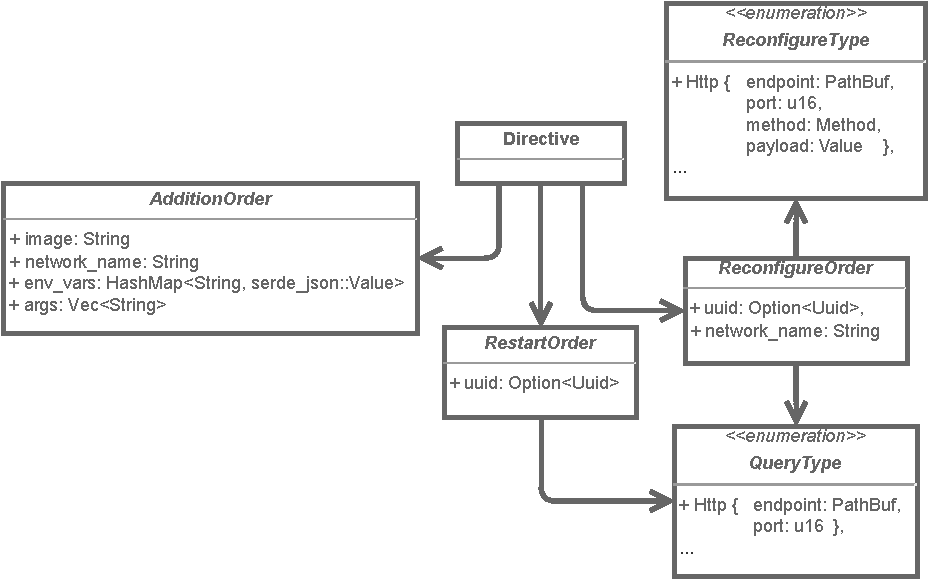
\includegraphics[width=0.85\linewidth]{images/Directives.pdf}
\end{figure}

Cada una estas directivas, y ordenes, se agregan a un registro en \textit{Bran}, usando el nombre de la aplicación y la locación a la pertenecen para su indexación. Cada una se registra usando un endpoint dedicado a la recepción de las órdenes.

La orden de adición contiene el nombre de la imagen del servicio a desplegar, la red a la cual debe conectarse para poder interactuar con los demás servicios, y los argumentos que se deben pasar sea como variables de ambiente o argumentos de línea de comando. 

Las órdenes de reinicio y reconfiguración poseen el \textit{UUID} del dispositivo que buscan afectar. Siendo así, al ser necesario tener una manera por la cual identificar qué servicio es qué componente, se implementó el enum \texttt{QueryType}. Este, contiene la información de como debe buscarse el contenedor en la red. Para esta primera implementación, su única variante es una búsqueda \textit{Http} hacia un endpoint y un puerto.

Finalmente, la orden de reconfiguración tiene como parte extra la red en la que se buscara el servicio a reiniciar y el tipo de reconfiguración (\texttt{ReconfigureType}) a realizar. Este funciona de manera similar a QueryType, en tanto indica la manera en la que se aplicará la reconfiguración. En este caso, para la variante \textit{Http} implementada, indica el endpoint y el puerto a usar, junto con el método y payload que deben ir en la petición para hacer la reconfiguración efectiva.

Se ha de resaltar que, estas ordenes, aunque contienen las instrucciones para poder realizar modificaciones a la arquitectura, en el momento de su declaración, no están completas y requieren de información extra para poder ejecutarse.

El proceso de la figura \ref{fig:BranExecution}, muestra el proceso por el cual las órdenes presentes en el registro de directivas de \textit{Bran}, son usadas como base para la construcción de las órdenes finales, y son enviadas para su posterior ejecución.

\begin{figure}[ht]
    \centering
    \caption{\\Proceso de decisión de acciones base realizado por Bran}
    \label{fig:BranExecution}
    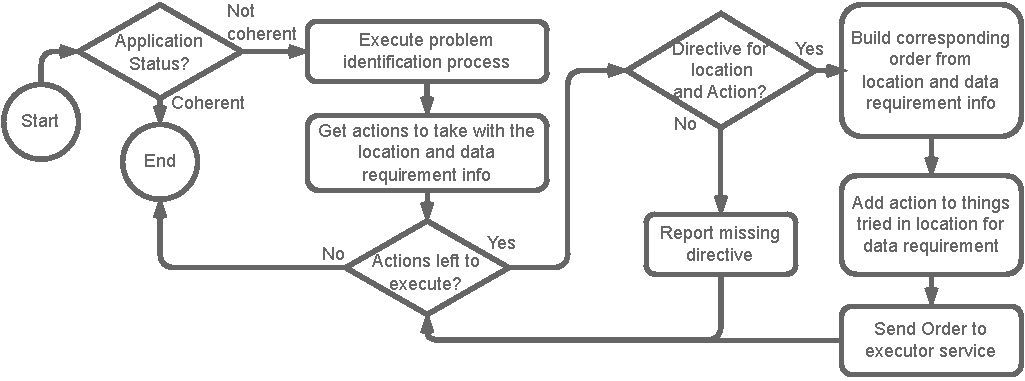
\includegraphics[width=0.9\linewidth]{images/BranProcessExecuter.pdf}
\end{figure}

Su ejecución inicia validando el estado de la aplicación reportada. En caso de este sea diferente a \textit{Coherent}, se llamará al proceso de identificación de problemas para obtener las acciones a realizar para alterar el estado de aplicación.

Una vez recibido el vector conteniendo las acciones, y la información asociada correspondiente, se realizará la construcción de cada una de las órdenes a ejecutar. Esta construcción se realiza a partir de las instrucciones bases establecidas en las directivas usando el UUID para las acciones de \textit{Restart} y \textit{Reconfigure}; y la información de la locación y el requerimiento de dato en las acciones de \textit{Addition}\footnote{Es necesario resaltar que estas construcciones, en especial para el caso de las acciones de \textit{Addition}, fueron implementadas para funcionar con los servicios \textit{Mocker} desarrollados específicamente para el proyecto. Esto se explorará más a fondo durante la sección \ref{sec:experimental} y \ref{sec:future}.}. 

Ya con las ordenes creadas, estas se enviaran al servicio encargado de ejecutar las instrucciones, dando como como resultado, modificaciones en la arquitectura.
